In questa appendice mostreremo un esempio completo di utilizzo di \textit{DbN}, in particolare
l'esempio n.6 dell'articolo \citetitle{ProbOfEx} \cite{ProbOfEx} con la seguente 
$ KB = (\mathcal{T},\mathcal{A}) $

$ \mathcal{T}Box $ :
\begin{itemize}
	\item[] $ Bipolar \sqsupseteq Depressed $
	\item[] $ \mathbf T(Depressed) \sqsupseteq_{0.85} \neg\exists hasSymptom.MoodReactivity $
	\item[] $ \mathbf T(Bipolar) \sqsupseteq_{0.70} \exists hasSymptom.MoodReactivity $
	\item[] $ \mathbf T(ProstateCancerPatient) \sqsupseteq_{0.60} \exists hasSymptom.MoodReactivity $
	\item[] $ \mathbf T(ProstateCancerPatient) \sqsupseteq_{0.80} \exists hasSymptom.Nocturia $
	\item[] $ \mathbf T(Depressed) \sqsupseteq_{0.60} \exists Smart $
\end{itemize}
$\mathcal{A}Box $ :
\[ \{ Depressed(Greg), \neg Smart(Greg) \} \]
Set of \textit{Symptoms} $\mathcal{V} $:
\[ \{ \exists hasSymptom.MoodReactivity(Greg) \} \]
Set of Cost of Disease with \textit{Tipicality}:
\[ \{ Bipolar: 1000, ProstateCancerPatient: 10000, Depressed: 3000 \} \]

Output dello strumento con la seguente ontologia; passo 1, 
verifica della condizione $ KB \cup \mathcal{V} \equiv $ consistente:
\begin{minted}{text}
========== Adding a set of Symptoms to the KB ==========
Sintomo aggiunto: Greg MoodReactivity
========== Checking consistency ==========
========== The ontology is consistent ==========
\end{minted}
passo 2, generazione scenari possibili:
\begin{minted}{text}
INIZIO SCENARIO 1
Typical(Bipolar),Greg,0.7
Probabilità scenario: 0.364
FINE SCENARIO 1

INIZIO SCENARIO 2
Typical(ProstateCancerPatient),Greg,0.48
Probabilità scenario: 0.144
FINE SCENARIO 2

INIZIO SCENARIO 3
Typical(Bipolar),Greg,0.7
Typical(ProstateCancerPatient),Greg,0.48
Probabilità scenario: 0.3356
FINE SCENARIO 3
\end{minted}
passo 3, per ogni scenario si effettua l'inferenza, viene mostrato il primo come esempio:
\begin{minted}{text}

ONTOLOGIA PRIMA DELLA LETTURA DELLA QUERY
=================================
Greg member_of Depressed
Greg member_of Not(Smart)
Bipolar is_a [ontoBase.Depressed, owl.Thing]
Bipolar1 is_a [owl.Thing, ontoBase.r1.only(Not(ontoBase.Bipolar) & ontoBase.Bipolar1)]
IntersectionBipolarBipolar1 is_a [ontoBase.MoodReactivity, owl.Thing]
NotBipolar1 is_a [owl.Thing, ontoBase.r1.some(ontoBase.Bipolar & ontoBase.Bipolar1)]
......
=================================
FINE ONTOLOGIA PRIMA DELLA LETTURA DELLA QUERY

LETTURA SINTOMI
=================================
Sintomo aggiunto: Greg: MoodReactivity
=================================
LETTURA SINTOMI TERMINATA

TRADUCENDO LO SCENARIO: 
=================================
INIZIO SCENARIO
Bipolar,Greg,0.7; 
Probabilità scenario: 0.364
FINE SCENARIO
Membro tipico:
Greg is_a Bipolar
Greg is_a Bipolar1
Greg is_a IntersectionBipolarBipolar1
=================================
FINE TRADUZIONE SCENARIO

ONTOLOGIA CON SCENARIO E SINTOMI
=================================
Bipolar is_a [ontoBase.Depressed, owl.Thing]
MoodReactivity is_a [owl.Thing]
Not(MoodReactivity) is_a [owl.Thing]
.....
Greg member_of Depressed
Greg member_of MoodReactivity
Greg member_of Not(Smart)
Greg member_of Not(MoodReactivity)
Greg member_of Bipolar1
Greg member_of IntersectionBipolarBipolar1
=================================
FINE ONTOLOGIA CON SCENARIO E SINTOMI

Il fatto segue logicamente nel seguente scenario: 
INIZIO SCENARIO
Bipolar,Greg,0.7; 
Probabilità scenario: 0.364
FINE SCENARIO
\end{minted}
passo 4, elenco degli scenari verificati e relativo grafico:
\begin{minted}{text}
RISULTATI DELL'INTERROGAZIONE: 
SCENARI IN CUI LA QUERY SEGUE LOGICAMENTE
INIZIO SCENARIO 1
Bipolar,Greg,0.7; 
Probabilità complessiva dello scenario: 0.364
FINE SCENARIO 1

INIZIO SCENARIO 2
ProstateCancerPatient,Greg,0.48; 
Probabilità complessiva dello scenario: 0.14400000000000002
FINE SCENARIO 2

INIZIO SCENARIO 3
Bipolar,Greg,0.7; ProstateCancerPatient,Greg,0.48; 
Probabilità complessiva dello scenario: 0.33599999999999997
FINE SCENARIO 3

PROBABILITÀ TOTALE: 0.844

Fine simulazione, tempo totale:  1.984983205795288  s
\end{minted}

\begin{figure}
	\centering
	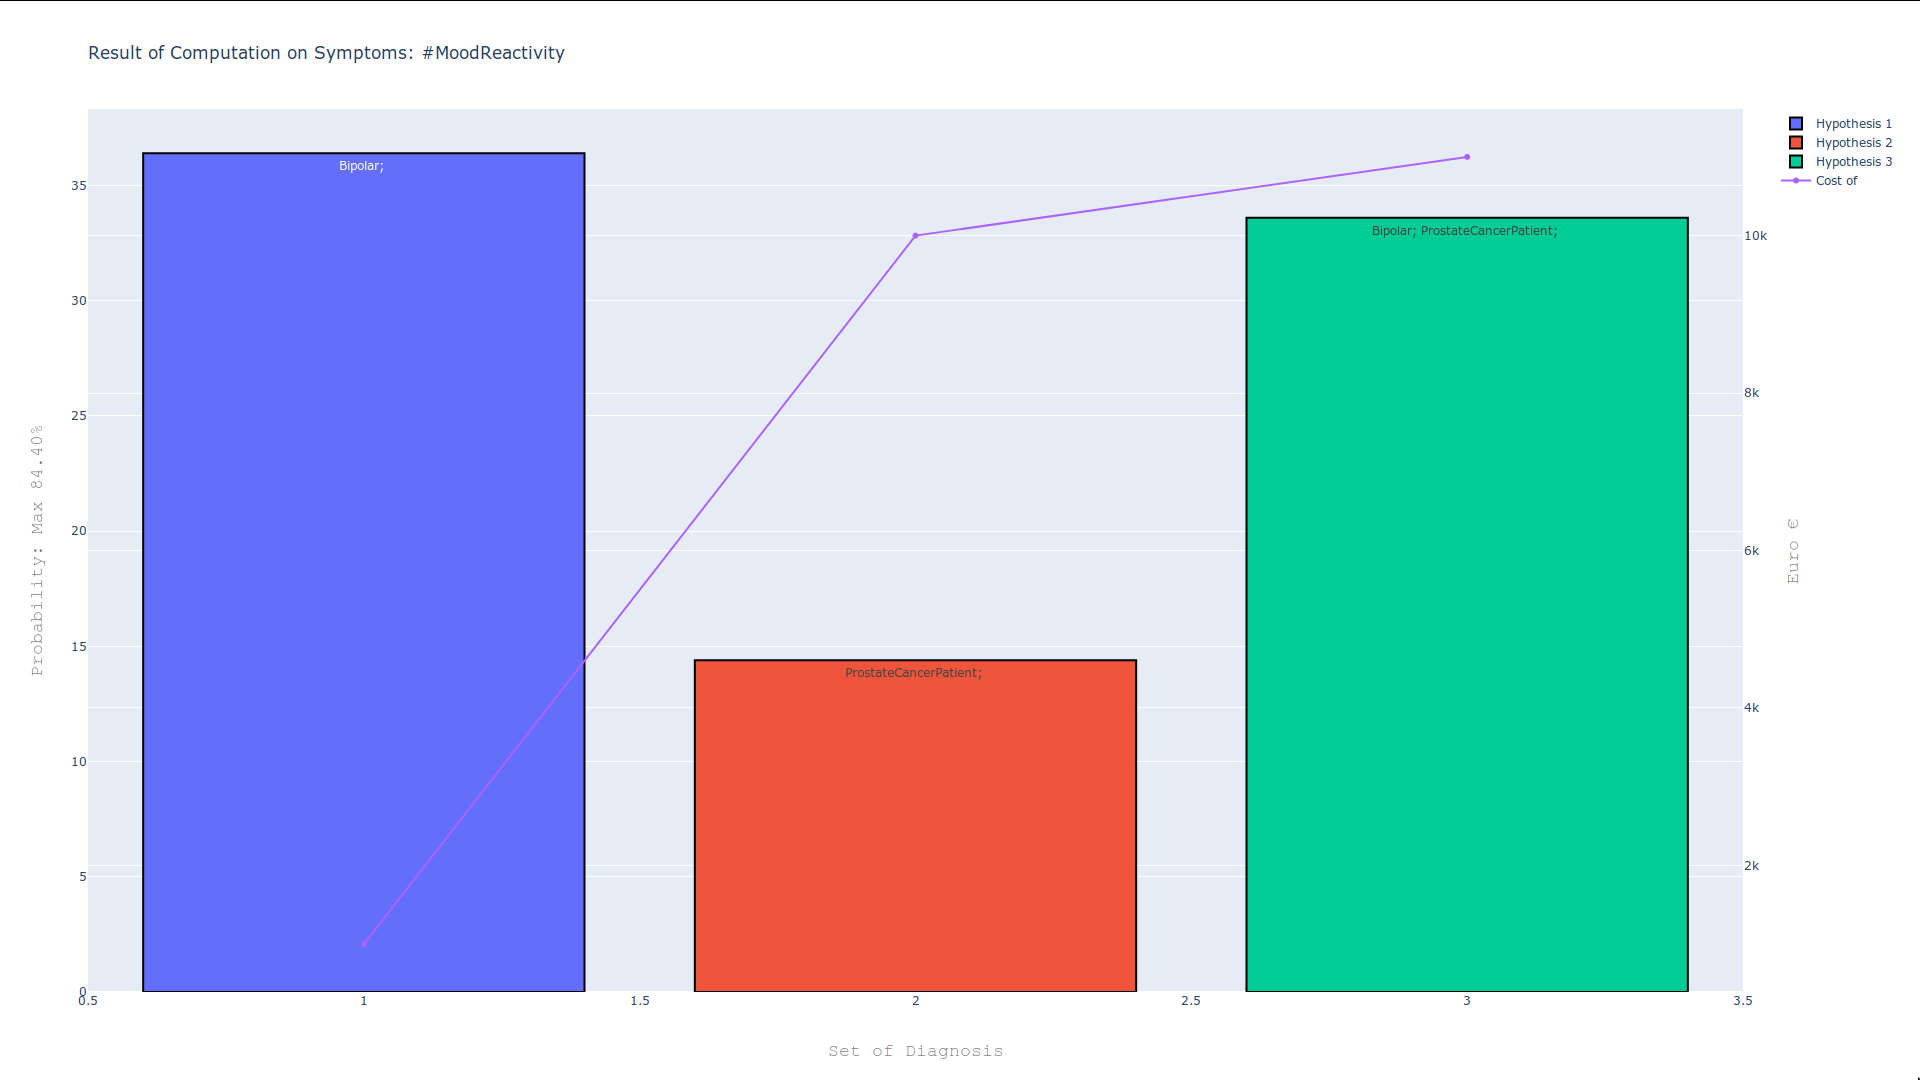
\includegraphics[width=\linewidth]{plot/Caso_di_studio.png}
	\caption{Versione Web}
\end{figure}

\begin{figure}
	\centering
	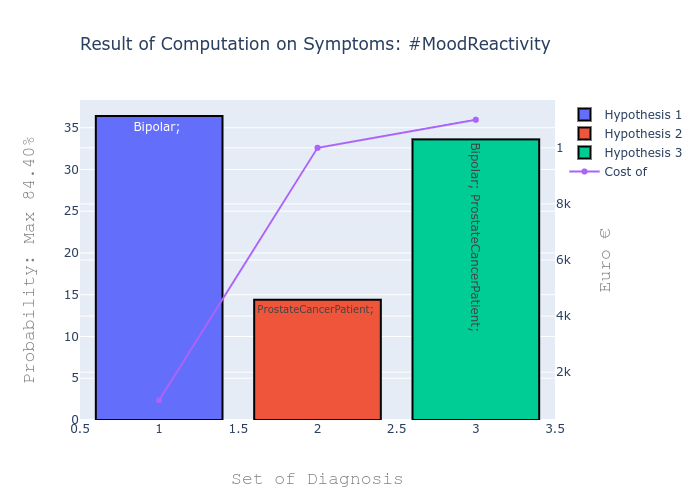
\includegraphics[width=\linewidth]{plot/caso_di_studio_alt.png}
	\caption{Versione documento}
\end{figure}